\documentclass[11pt]{article}
%\documentclass[11pt]{revtex4}
\usepackage{graphicx}
\usepackage{amssymb}
%\usepackage[]{epsfig}
%\usepackage{parskip}


\textheight 8.0in
\topmargin 0.0in
\textwidth 6.0in
\oddsidemargin 0.25in
\evensidemargin 0.25in

\newcommand{\gev}{\mathrm{GeV}}
\newcommand{\gevc}{\mathrm{GeV/c}}
\newcommand{\gevcc}{\mathrm{GeV/c^2}}
\newcommand{\mevcc}{\mathrm{MeV/c^2}}
\newcommand{\gevccgevcc}{\mathrm{GeV^2/c^4}}

\begin{document}


\title{Introduction to the {\tt AmpTools} Package\\ using the Dalitz Tutorial}
\author{Ryan Mitchell}
\date{\today}
\maketitle 

\begin{abstract}
This document introduces several of the core features of the {\tt AmpTools} package using a simplified Dalitz analysis as an example.  The Dalitz tutorial shows how to use the {\tt AmpTools} package to generate Monte Carlo distributions, write amplitudes, fit data, and plot the results.
\end{abstract}

%\maketitle

\tableofcontents

\parindent 0pt
\parskip 10pt


\section{Introduction}

The {\tt AmpTools} package is a versatile set of tools that allows a user to define custom amplitudes, which can then be used to generate Monte Carlo distributions, to fit data, and to make plots, among other tasks.  As the tools are both physics and experiment agnostic, the user has the freedom to write applications that are highly customizable.  But in return, the user must provide a number of derived classes to write data to files (Section~\ref{sec:dw}: {\tt DalitzDataIO/DalitzDataWriter}), to read data from files (Section~\ref{sec:dr}: {\tt DalitzDataIO/ DalitzDataReader}), to calculate amplitudes (Section~\ref{sec:bw}: {\tt DalitzAmp/BreitWigner}), and to plot fit results (Section~\ref{sec:dpg}: {\tt DalitzPlot/DalitzPlotGenerator}).  The Dalitz tutorial provides a simple example, from beginning to end, of how to write these derived classes, and how to then build executables from the resulting libraries.

The Dalitz tutorial considers a fictitious decay of a $3.0~\gevcc$ particle to three $200~\mevcc$ particles.  Two-body Breit-Wigner distributions are used to illustrate amplitude construction.

This tutorial could be used as a starting point for new analyses.  It is recommended that the steps presented here are followed consecutively to gradually build up an analysis from simply reading in data to fitting data and plotting the results.



\section{Preliminaries}

Two external packages are required to run the Dalitz tutorial: {\tt ROOT} and {\tt CLHEP}. Once they are installed (directions for installation can be found elsewhere), the following environment variables should be set:
\begin{verbatim}
  > setenv ROOTSYS [top ROOT directory]
  > setenv CLHEP_INCLUDE_DIR [directory of CLHEP header files]
  > setenv CLHEP_LIB_DIR [directory of CLHEP libraries]
\end{verbatim}

The latest fixed release of the {\tt AmpTools} code, along with related packages and tutorials, can be downloaded as a tarball from {\tt sourceforge.net/projects/amptools}.  Once unpacking the tarball, set the following:
\begin{verbatim}
  > setenv AMPTOOLS [top directory]/AmpTools
  > setenv AMPPLOTTER [top directory]/AmpPlotter
  > setenv DALITZ [top directory]/Tutorials/Dalitz
\end{verbatim}

The {\tt \$AMPTOOLS} directory contains the source code for the {\tt AmpTools} framework;  {\tt \$AMPPLOTTER} contains code for a GUI to view fit results; and {\tt \$DALITZ} contains the Dalitz tutorial to be discussed in this document.  To compile these, the following should work (after perhaps modifying Makefiles to account for different computing platforms):
\begin{verbatim}
  > cd $AMPTOOLS
  > make
  > cd $AMPPLOTTER
  > make
  > cd $DALITZ
  > make
\end{verbatim}


\section{Directory Structure}

The Dalitz tutorial package contains a number of subdirectories.  Three of these directories include class definitions that are derived from {\tt AmpTools} classes:
\begin{itemize}
\item {\tt \bf DalitzDataIO}:  This directory holds custom classes to read and write data.  The {\tt DalitzDataWriter} class is derived from the {\tt DataWriter} class of {\tt AmpTools}, and the {\tt DalitzDataReader} class is derived from the {\tt DataReader} class.  They are used to read and write data in a custom {\tt ROOT} tree format.
\item {\tt \bf DalitzAmp}: This directory holds user-defined amplitudes derived from the {\tt Amplitude} class of {\tt AmpTools}.  The {\tt BreitWigner} class is a simple example of such an amplitude.
\item {\tt \bf DalitzPlot}:  This directory holds the {\tt DalitzPlotGenerator} class, which is derived from the {\tt PlotGenerator} class of {\tt AmpTools}.  This class holds instructions for making custom plots of fit results.
\end{itemize}

Libraries are generated from these derived classes and placed in a {\tt lib} directory by using the {\tt Makefile} in the top directory (as above):
\begin{verbatim}
  > cd $DALITZ
  > make
\end{verbatim}

Other directories include examples of how to use these libraries to build and run executables:
\begin{itemize}
\item {\tt \bf DalitzExe}:  This directory holds example code that can be used to build executables from the libraries generated above.  Each executable is described in later sections.
\item {\tt \bf run}:  This directory is used to run executables.
\end{itemize}
Note that the {\tt DalitzExe} and {\tt run} directories could be separated from the other directories.  

To build executables, for example the {\tt generatePhaseSpace} executable, the {\tt Makefile} in the {\tt DalitzExe} directory can be used:
\begin{verbatim}
  > cd $DALITZ/DalitzExe
  > make generatePhaseSpace_exe
\end{verbatim}

Alternatively, all of the executables can be built at once:
\begin{verbatim}
  > cd $DALITZ/DalitzExe
  > make
\end{verbatim}

\section{Setting up a Data Writer: \\ 
{\tt DalitzDataIO/DalitzDataWriter}}
\label{sec:dw}

The main purpose of a {\tt DataWriter} class in {\tt AmpTools} is to take a {\tt Kinematics} object, which contains four-vectors, and write its contents to an output file.  The user must write a class derived from the {\tt DataWriter} class to customize the output, including the format of the output file, the variables to be written, and so on.  In the {\tt DalitzDataWriter} example, output files are in a {\tt ROOT} tree format and contain the four-vectors of the three fictitious final state particles of the Dalitz tutorial.

\section{Generating Phase Space: \\  
{\tt DalitzExe/generatePhaseSpace}}
\label{sec:ps}

The {\tt generatePhaseSpace} application is an example of how to use the {\tt DalitzDataWriter} to write data to an output file.  It makes use of the {\tt TGenPhaseSpace} class from {\tt ROOT}.  A fictitious decay of a particle with mass $3.0~\gevcc$ to three $200~\mevcc$ particles is used for illustration.  To compile and run the example, use:
\begin{verbatim}
  > cd $DALITZ/DalitzExe
  > make generatePhaseSpace_exe
  > cd $DALITZ/run
  > $DALITZ/DalitzExe/generatePhaseSpace phasespace.gen.root 100000
\end{verbatim}
This will make a file called {\tt phasespace.gen.root} with 100000 events generated according to phase space.

\section{Setting up a Data Reader: \\
{\tt DalitzDataIO/DalitzDataReader}}
\label{sec:dr}

The {\tt DataReader} class in {\tt AmpTools} is designed to read data from an input file and pack it into a {\tt Kinematics} object, which can then be distributed to other classes or applications.  The user must write a class deriving from the {\tt DataReader} class to customize the data format (which should match the format written by the {\tt DataWriter}).  The {\tt DalitzDataReader} is an example that can read the output files from the {\tt DalitzDataWriter}.

\section{Making Plots: \\
{\tt DalitzExe/plotData}}
\label{sec:plot}

The {\tt plotData} executable is an example that uses the {\tt DalitzDataReader} to read events from an input file and then makes histograms of kinematic variables using {\tt ROOT}.  To compile and run, use:
\begin{verbatim}
  > cd $DALITZ/DalitzExe
  > make plotData_exe
  > cd $DALITZ/run
  > $DALITZ/DalitzExe/plotData phasespace.gen.root plots.phasespace.gen.root
\end{verbatim}
This will read the input file {\tt phasespace.gen.root} (generated in Section~\ref{sec:ps}) and output a file of histograms called {\tt plots.phasespace.gen.root}.  Histograms can be viewed in {\tt ROOT} using, for example:
\begin{verbatim}
  > cd $DALITZ/run
  > root plots.phasespace.gen.root
  root>  hs12s23->Draw("colz")
\end{verbatim}
The resulting histogram is shown in Figure~\ref{fig:dalitz}a.

\begin{figure}[h!]
\begin{center}
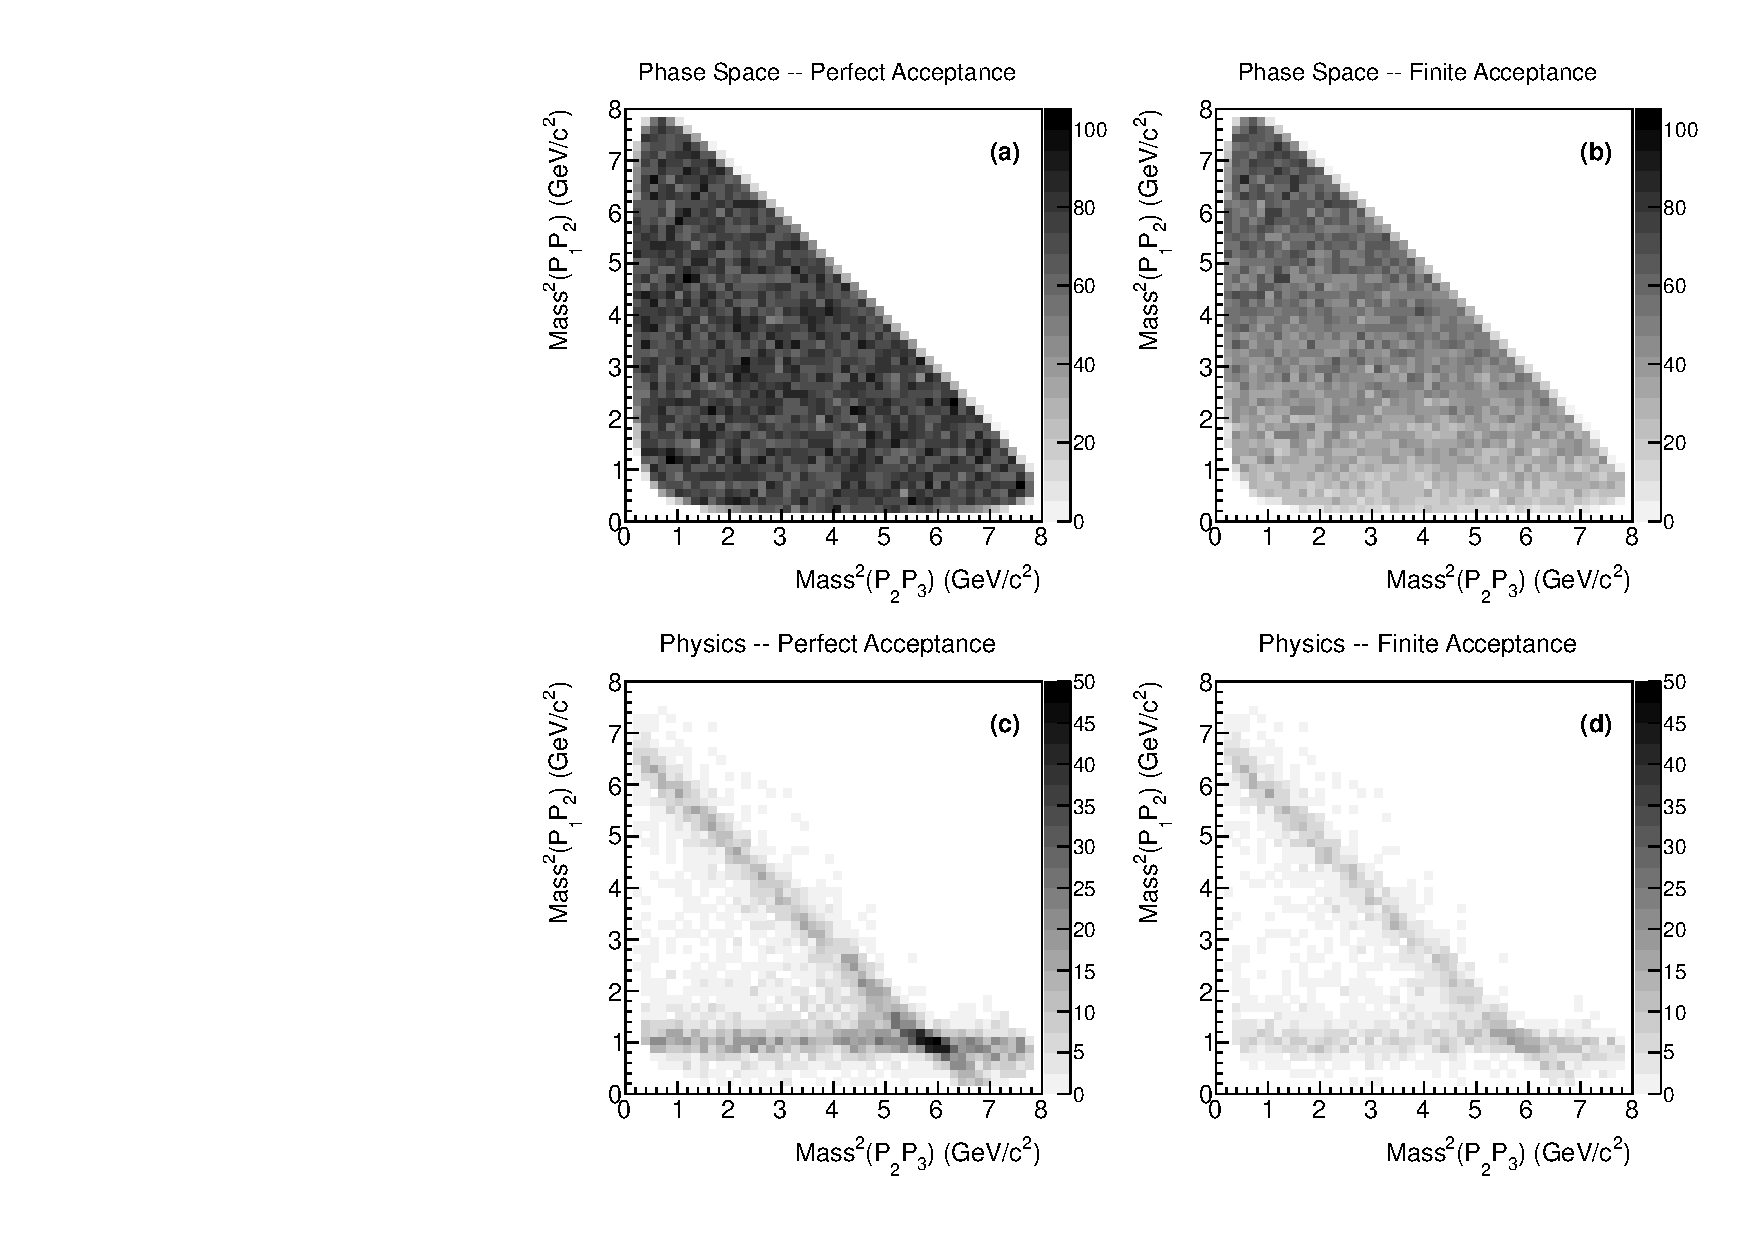
\includegraphics[width=1.0\columnwidth]{figure1.pdf}
\caption{Dalitz distributions for a $3.0~\gevcc$ particle decaying to three $200~\mevcc$ particles.  Plots were generated using the {\tt plotData} executable with input data files described in the text.
\label{fig:dalitz}}
\end{center}
\end{figure}


\section{Simulating Detector Effects: \\
{\tt DalitzExe/toyAcceptance}}
\label{sec:eff}

The {\tt toyAcceptance} example uses the {\tt DalitzDataReader} to read events from an input file, accepts or rejects events based on a toy efficiency function, then writes the accepted events to an output file using the {\tt DalitzDataWriter}.  Here is an example of how to compile and run:
\begin{verbatim}
  > cd $DALITZ/DalitzExe
  > make toyAcceptance_exe
  > cd $DALITZ/run
  > $DALITZ/DalitzExe/toyAcceptance phasespace.gen.root phasespace.acc.root
\end{verbatim}
This takes the input file {\tt phasespace.gen.root} (generated in Section~\ref{sec:ps}) and outputs a file called {\tt phasespace.acc.root} containing events that survive the toy simulation.

To view the resulting kinematic distributions, one can use the {\tt plotData} application described in Section~\ref{sec:plot}:
\begin{verbatim}
  > cd $DALITZ/run
  > $DALITZ/DalitzExe/plotData phasespace.acc.root plots.phasespace.acc.root
\end{verbatim}
The resulting Dalitz plot is shown in Figure~\ref{fig:dalitz}b.


\section{Setting up an Amplitude: \\
{\tt DalitzAmp/BreitWigner}}
\label{sec:bw}

One of the most important aspects of the {\tt AmpTools} package is the flexibility it offers in defining physics amplitudes.  The user must write amplitude classes that derive from the {\tt Amplitude} class.  The {\tt BreitWigner} class (found in the {\tt DalitzAmp} directory) is a simple example.  Pay special attention to the {\tt calcAmplitude} method, where the amplitude is actually calculated.

\section{Setting up a Configuration File: \\
{\tt run/dalitz1.cfg}}
\label{sec:config}



The {\tt AmpTools} package uses the {\tt AmplitudeManager} class to manage amplitudes.  As there are many steps in initializing an {\tt AmplitudeManager}, configuration files (parsed by the {\tt ConfigFileParser} class) can be used to simplify the process.  Configuration files can be used to define which amplitudes should be used, how they should be combined (coherently or incoherently, for example), what the free parameters are, their initial values, and so on.  A simple example is the {\tt dalitz1.cfg} file found in the {\tt run} directory of the Dalitz tutorial.  This example defines two Breit-Wigner amplitudes: one of mass $1.0~\gevcc$ decaying to particles~1 and~2; and one of mass $1.5~\gevcc$ decaying to particles~1 and~3.  See the top of the {\tt dalitz1.cfg} file for a list of commands that can be used in configuration files.

\section{Parsing a Configuration File: \\
{\tt DalitzExe/parseConfigFile}}

The {\tt parseConfigFile} application is a simple example showing how to parse a configuration file using the {\tt ConfigFileParser} class, and then display the configuration information to the screen.  This is a useful way to make sure there are no mistakes in a configuration file.  To compile and run, use:
\begin{verbatim}
  > cd $DALITZ/DalitzExe
  > make parseConfigFile_exe
  > cd $DALITZ/run
  > $DALITZ/DalitzExe/parseConfigFile dalitz1.cfg
\end{verbatim}
This parses and displays information from the {\tt dalitz1.cfg} file found in the {\tt run} directory.  The {\tt dalitz3.cfg} file is a more complicated configuration file that includes additional free parameters:
\begin{verbatim}
  > $DALITZ/DalitzExe/parseConfigFile dalitz3.cfg
\end{verbatim}

\section{Printing Amplitude Values: \\
{\tt DalitzExe/printAmplitudes}}

The {\tt printAmplitudes} example parses a configuration file using the {\tt ConfigFileParser}, reads in events using the {\tt DalitzDataReader}, sets up an {\tt AmpToolsInterface}, calculates {\tt BreitWigner} amplitudes and total intensities, and then prints amplitude and intensity values to the screen. This can be a useful way to make sure amplitudes are coded correctly.  Compile and run in the usual way:
\begin{verbatim}
  > cd $DALITZ/DalitzExe
  > make printAmplitudes_exe
  > cd $DALITZ/run
  > $DALITZ/DalitzExe/printAmplitudes dalitz1.cfg phasespace.gen.root
\end{verbatim}
This takes as input the {\tt dalitz1.cfg} configuration file~(Section~\ref{sec:config}) and the data file {\tt phasespace.gen.root}~(Section~\ref{sec:ps}).

\section{Generating Physics Distributions: \\ 
{\tt DalitzExe/generatePhysics}}
\label{sec:physics}

The {\tt generatePhysics} example generates events according to amplitudes specified in a configuration file.  To do so, it parses a configuration file using the {\tt ConfigFileParser}, sets up an {\tt AmpToolsInterface}, generates phase space events using the {\tt TGenPhaseSpace} class from {\tt ROOT}, calculates intensities from those events and uses an accept/reject method to mimic the desired physics distribution, then writes the resulting events to a data file using a {\tt DalitzDataWriter}.  To compile and run, use:
\begin{verbatim}
  > cd $DALITZ/DalitzExe
  > make generatePhysics_exe
  > cd $DALITZ/run
  > $DALITZ/DalitzExe/generatePhysics dalitz1.cfg physics.gen.root 100000
\end{verbatim}
This inputs the {\tt dalitz1.cfg} configuration file~(Section~\ref{sec:config}), outputs a data file called {\tt physics.gen.root}, and does accept/reject starting with 100000 phase space events.

The {\tt toyAcceptance} executable can be used on the output file to simulate the effects of a finite acceptance:
\begin{verbatim}
  > $DALITZ/DalitzExe/toyAcceptance physics.gen.root physics.acc.root
\end{verbatim}
Finally, histograms can be produced from both the generated and accepted data files using the {\tt plotData} executable:
\begin{verbatim}
  > $DALITZ/DalitzExe/plotData physics.gen.root plots.physics.gen.root
  > $DALITZ/DalitzExe/plotData physics.acc.root plots.physics.acc.root
\end{verbatim}
The results are shown in Figures~\ref{fig:dalitz}c and~\ref{fig:dalitz}d, respectively.

\section{Fitting Amplitudes: \\
{\tt DalitzExe/fitAmplitudes}}
\label{sec:fit}

Amplitudes can be fit to data following the {\tt fitAmplitudes} example.  The example shows how to set up an {\tt AmpToolsInterface} class, perform a fit, and then output results to a text file:
\begin{verbatim}
  > cd $DALITZ/DalitzExe
  > make fitAmplitudes_exe
  > cd $DALITZ/run
  > $DALITZ/DalitzExe/fitAmplitudes dalitz1.cfg
\end{verbatim}
This takes a configuration file {\tt dalitz1.cfg} as input and outputs a text file with results called {\tt dalitz1.fit}.  The configuration file specifies that the fit is done to data in the file {\tt physics.acc.root}~(Section~\ref{sec:physics}), and the acceptance is evaluated using the files {\tt phasespace.gen.root}~(Section~\ref{sec:ps}) and {\tt phasespace.acc.root}~(Section~\ref{sec:eff}).

Fits using other example configuration files can also be performed.  The {\tt dalitz2.cfg} configuration file corresponds to a case with perfect acceptance.  The {\tt dalitz3.cfg} configuration file lets the masses and widths of the resonances float.

\section{Setting up a Plot Generator: \\
{\tt DalitzPlot/DalitzPlotGenerator}}
\label{sec:dpg}

To use the results of a fit to make plots, a user can write a class that derives from the {\tt PlotGenerator} class of the {\tt AmpTools} package.  The {\tt DalitzPlotGenerator} (found in the {\tt DalitzPlot} directory) is an example of how to do this.  Plots are generated for data, acceptance-corrected fit results, and acceptance-uncorrected fit results.  To visualize the quality of the fit over certain projections of the data, one can compare the data plots with the acceptance-uncorrected fit plots.  Plots of fit results using only single amplitudes are also constructed and can be used to visualize the contributions of individual amplitudes.


\section{Plotting Fit Results: \\
{\tt DalitzExe/plotResults}}

The {\tt plotResults} application uses the {\tt DalitzPlotGenerator} to make {\tt ROOT} histograms from fit results.  Compile and run it like this:
\begin{verbatim}
  > cd $DALITZ/DalitzExe
  > make plotResults_exe
  > cd $DALITZ/run
  > $DALITZ/DalitzExe/plotResults dalitz1.cfg dalitz1.fit dalitz1.root
\end{verbatim}
This takes as input the {\tt dalitz1.cfg} configuration file and the {\tt dalitz1.fit} text file containing fit results~(Section~\ref{sec:fit}).  The output is {\tt dalitz1.root}, a {\tt ROOT} file containing histograms.

To plot data with fit results overlaid, one can use, for example:
\begin{verbatim}
  > root dalitz1.root
  root>  hm12dat->Draw("e")
  root>  hm12acc->Draw("hist,same")
  root>  hm12acc1->Draw("hist,same")
  root>  hm12acc2->Draw("hist,same")
\end{verbatim}
The {\tt hm12acc1} and {\tt hm12acc2} histograms show the contributions of the first and second amplitudes, respectively.  Similarly, for the acceptance-corrected results, one could use:
\begin{verbatim}
  > root dalitz1.root
  root>  hm12gen->Draw("hist")
  root>  hm12gen1->Draw("hist,same")
  root>  hm12gen2->Draw("hist,same")
\end{verbatim}

Results are shown in Figure~\ref{fig:results}.

\newpage
\begin{figure}[h!]
\begin{center}
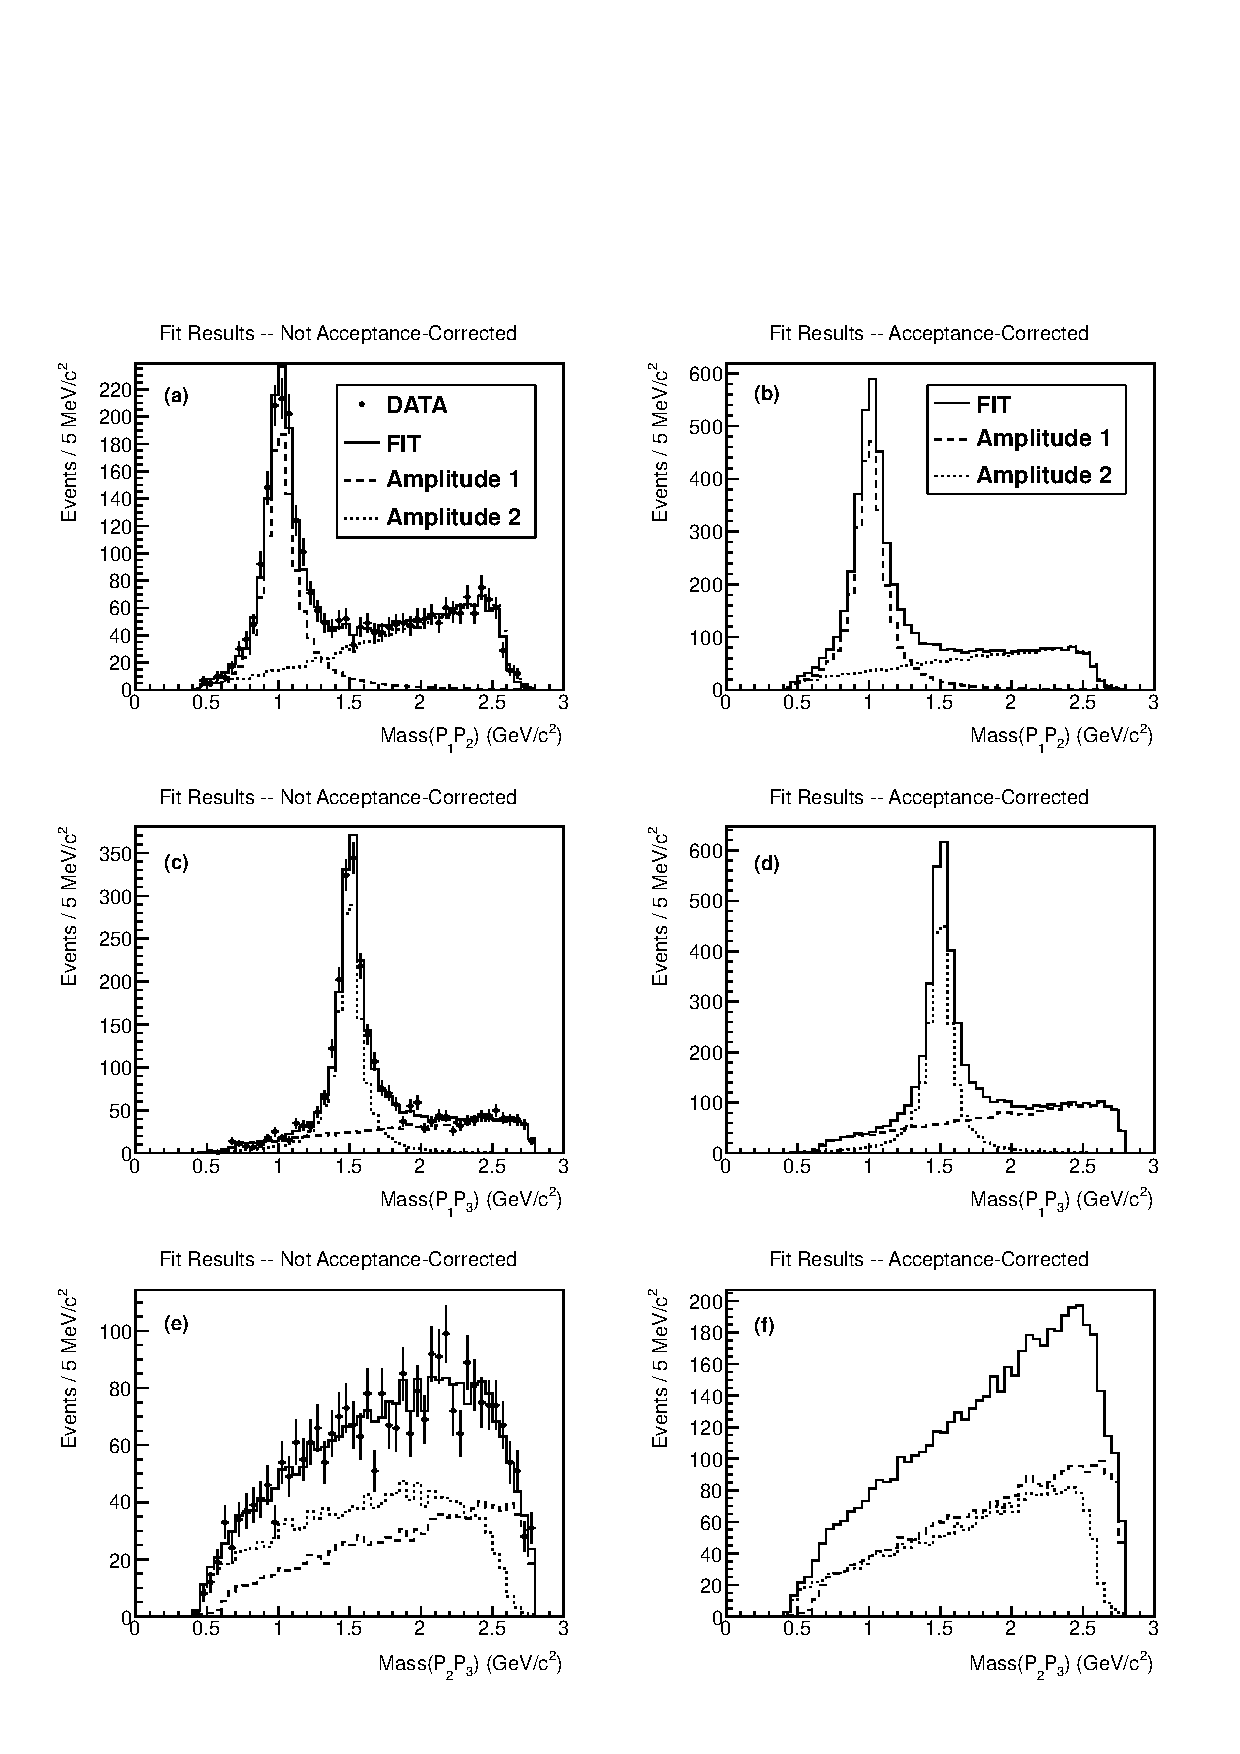
\includegraphics[width=1.0\columnwidth]{figure2.pdf}
\caption{Fit results.  The left column shows a comparison of data with fit results not corrected for acceptance effects.  The right column shows the acceptance-corrected fit results.  (a-b)~Projection onto $M(P_1P_2)$.  (c-d)~Projection onto $M(P_1P_3)$.  (e-f)~Projection onto $M(P_2P_3)$.
\label{fig:results}}
\end{center}
\end{figure}

\end{document}
